\documentclass{article}
\usepackage[UTF8]{ctex}
\usepackage{geometry}
\usepackage{natbib}
\geometry{left=3.18cm,right=3.18cm,top=2.54cm,bottom=2.54cm}
\usepackage{graphicx}
\pagestyle{plain}	
\usepackage{setspace}
\usepackage{caption2}
\usepackage{datetime} %日期
\renewcommand{\today}{\number\year 年 \number\month 月 \number\day 日}
\renewcommand{\captionlabelfont}{\small}
\renewcommand{\captionfont}{\small}
\begin{document}

\begin{figure}
    \centering
    
\includegraphics[width=8cm]{upc.png}

    \label{figupc}
\end{figure}

	\begin{center}
		\quad \\
		\quad \\
		\heiti \fontsize{45}{17} \quad \quad \quad 
		\vskip 1.5cm
		\heiti \zihao{2} 《信息技术前沿讲座》课程总结报告
	\end{center}
	\vskip 2.0cm
		
	\begin{quotation}
% 	\begin{center}
		\doublespacing
		
        \zihao{4}\par\setlength\parindent{7em}
		\quad 

		学生姓名:\underline{\qquad  张凯文 \qquad \qquad}

		学\hspace{0.61cm} 号:\underline{\qquad 1808010407\qquad}
		
		专业班级:\underline{\qquad 计科1804 \qquad  }
		
        学\hspace{0.61cm} 院:\underline{计算机科学与技术学院}
% 	\end{center}
		\vskip 2cm
		\centering
		\begin{table}[h]
            \centering 
            \zihao{4}
            \begin{tabular}{|c|c|c|c|c|c|}
            % 这里的rl 与表格对应可以看到,姓名是r,右对齐的;学号是l,左对齐的;若想居中,使用c关键字。
                \hline
                课程认识 & 问题思 考 & 格式规范  & Latex文档制作   & 总分 & 评阅教师 \\
                30\% & 30\% & 20\% & 20\%  &  &  \\
                \hline
                 & & & &  &\\
                & & & &  &\\
                \hline
            \end{tabular}
        \end{table}
		\vskip 2cm
		\today
	\end{quotation}

\thispagestyle{empty}
\newpage
\setcounter{page}{1}
% 在这之前是封面,在这之后是正文
\section{引言}
在老师的悉心指导下,《信息技术前沿讲座》课程已落下帷幕。虽然课时不多,但是让我深刻理解了很多道理,比如对自己受益终生的道理改革开、放这段时间的大事,中美、中日之间的关系以及国际与国内的百年未有之大变局。既增长了许多知识,又丰富了自己的阅历,受益良多。

\section{认识与体会}
首先谈一下个人对课程的整体认识:我觉得我可以把我理解到的内容概括为两个方面。一个是个人,另一个是国家。第一章李运华的额案例和第二章求职者的简历可以转化为个人对自己勉励,怎样成为大牛、怎样获得更好的职位,这些都是我们这些大学生应该思考的,就像老师说的那样,现在是二年级,已经到了思考这些问题的时候了。怎样让自己以后的路走的更加顺畅,这个问题只有自己才能合适的答案。而第三章中,老师分析了新一代信息技术革命的背景、内涵及其应用,在这一部分我感触较深的就是百年未有之大变局。大变局,大在何处,变在何处,老师都给出了具体的分析,既有国内方面,又有国际局势,并且结合当下的疫情着重的分析了现在的国际局势,让我们有了更加深刻、更加明白的理解,从而可以做出更加准确的判断。下面我主要分享一下自己印象很深的几点。\par

%\subsection{这里是子标题样例}
%图片插入的样例:\par
%\begin{figure}[h!]
%\centering
%\includegraphics[scale=1.7]{universe}
%\caption{The Universe}
%\label{fig:universe}
%\end{figure}

%\subsection{第二个子标题}
%表格插入样例:\par
%
%\begin{table}[h]
%    \centering
%    \caption{这是科学系的花名册}
%\begin{tabular}{rl}
%% 这里的rl 与表格对应可以看到,姓名是r,右对齐的;学号是l,左对齐的;若想居中,使用c关键字。
%    \hline
%    姓名 & 学号 \\
%    \hline
%    张三 & 190704xxxx+++ \\ 
%    李四 & 190704yyyy \\
%    王二五 & 190704zzzz\\
%    \hline
%\end{tabular}
%    \label{table1}
%\end{table}
%\subsection{第三个子标题}
%这里是引用的样例:\par
%{\bf 注意,仅仅是引用的样例}\par
%我阅读了图书《机器学习实战》\citep{Harrington2013},引发了我对卷积神经网络的兴趣,于是阅读了期刊论文《卷积神经网络研究综述》\citep{zhoufeiyan},基于对卷积神经网络的深刻认识,我又学习了2018年计算机视觉领域的会议ECCV的会议论文《TextSnake》\citep{long2018textsnake},来探索深度学习落实在生活生产领域的实际意义。\par

%\subsection{这里是子标题样例}
第一章的大牛养成指南就使我感触颇多,李运华的事例让我更加深刻的意识到——吃的草够多,真的可能成为大牛。李运华的博文里写道:一鸣惊人的额背后是1万小时的不断练习。其实绝大多数成功人士的背后,都是一点点积累起来的,比如说他举的例子:莫扎特、甲壳虫乐队和比尔乔伊。莫扎特是众所周知的音乐神童,6岁就开始作曲,但是他真正出人头地是20多岁的时候,也就是说他虽然6岁开始作曲,但他当时作的曲也是比较不好的。莫扎特曾经这样描述他自己:“人们以为我的艺术得来全不费功夫。实际上,没有人会像我一样花这么多时间和思考来从事作曲;没有一位名家的作品我不是辛勤地研究了许多次。”他的成功绝不仅是世人口中的天才,天才是奋斗出来的.第二个是甲壳虫乐队,他们每天在酒吧里面演出8小时、10小时,演出了几年,后来发行专辑之后才一鸣惊人。第三个案例叫比尔乔伊,大家可能都知道比尔盖茨,但是不知道比尔.乔伊,他是UNIX天才的程序员,从伯克利大学开始,包括他后面的工作,进行了将近1万小时的编程,在80年代能够编1万小时的是凤毛麟角。其实在当下,遍1万小时也是出类拔萃的了。


成功不可能一蹴而就。美国作家杰克.伦敦的房间里有着各种奇形怪状的装饰,窗帘、衣架或者是厨具上,都挂着小纸片,每个纸片上都记录着一些优美的词汇,他在房间的每个角落都放上制片,目的便是每时每刻都能随时记诵,像比尔乔伊的一万小时一样,正是杰克伦敦这种对语言和素材的不断积累,他才能在后来的写作中得心应手,写出许多脍炙人口的佳作。不管你取得多大的成就,都离不开积累。这一点,我们的老祖宗就已经给我们解释了:“积土成山,风雨兴焉。积水成渊,风雨兴焉。积善成德,而神明自得,圣心备焉”,这便是《荀子》中的积累。现在谈人生还太早,但我还是想说,漫漫人生路其实就是一个不断积累的过程,从牙牙学语到出口成章,从青涩懵懂到风华正茂,从畏畏缩缩到勇往直前……这些都是积累。万丈高楼起于垒石,万里长征基于寸步,浩瀚林海生于棵棵大树——成功是积累起来的。


冰冻三尺非一日之寒。马克思在准备写《资本论》时,需要成册书籍1500多种,并且为此做的笔记就有250多本;列宁为了研究资本主义社会的法律,曾翻阅了数以百计的书籍,其中阅读了148本书和48种刊物上的两百多篇文章,并在此基础上,进行分析,批判,研究,随之完成了著作《帝国主义是资本主义的最高阶级》;爱迪生口袋里经常带着一个先笔记本,有事在上面画上草图,写下一些计算公式,这个笔记本就像他的知识宝典,时不时拿出来研究研究,这也就成就了“发明大王”的称号。由此可见,成功离不开点滴的积累。


再回到李运华介绍的一万小时理论,就像他自己说的那样,第一次看到一万小时的理论,觉得没有什么神奇的,他自己算了算,只需要五年他就能成为业界的大牛,但经过后来的反思他发现,这是很困难的,因为大多数人每天的工作其实是在重复劳动。那么这一万小时就意味着你每天要花三个小时用来提升自己的技能。这样一直坚持下去,要持续十年的时间。注意,是提升自己的技能而不是原地踏步,如果你拿一年的经验重复了九年,那纯粹是在浪费时间,我觉得,这便是那一万个小时的精髓。每天坚持学习三个小时,提升自己,可能有些人乍一看会觉得比较轻松,但我们来看一个非常明显的案例。苏格拉底让他的学生甩手臂的例子大家一定听说过,苏格拉底告诉他的学生,每天把手臂往前摆动300下,然后再往后摆动300下,看看谁能每天坚持下来。过了几天,苏格拉底上课的时候的让坚持的同学举手,结果有90%的同学举了手,过了一个月,他又让坚持下来的同学举手,这事只有70%的同学举了手,一年之后,他又同样要求,结果只有一个同学举手,也就是后来伟大的哲学家柏拉图。从这里我们也能看出,即便是像甩手臂这样简单机械的动作,坚持上一年也是非常罕见的,更不必说坚持上十年,而且每天都要花三个小时来提升自己,这更是难上加难。所以说,伟大,是熬出来的。


正如邓拓说的,真正所谓成就,就是在前人知识和经验的基础上有所发展,没有积累就什么也谈不上,注重积累,不断积累才能扎下深厚的学问之根。


有了一万小时的理论,但还有一个很现实的问题,时间从哪里来。在他的博文里,李运华介绍了他是怎样找到10000小时的:碎片化时间管理。首先是找到三个三十分钟:早上、睡觉前和上班到你座位上。其次是利用和节省路途时间,可以利用上下班的时间看书或者听书,或者是进行合理的投资,搬到离公司近的地方,虽然每个月会多出一部分房租的开支,但若是把剩下的时间用来提升自己,他最终的收益绝不是这些房租所能比得过的。最后就是周末的四个小时,就李运华而言,他通过周末挤出的四个小时,在一年之内,读了84本书,这种收获也是非常巨大的。这里有一个利用碎片化时间办成大事的故事:有两个和尚住在隔壁,所谓隔壁是隔壁那座山—他们分别在相邻的两座山上的庙里,这两座山之间有一条小溪于是这两人每天都会在同一时间下山挑水,久而久之,他们便成了朋友。就这样,时间在每天的挑水中,不知不觉的已经过了五年。突然有一天,左边这座山的和尚没有下山挑水,另一个和尚心想:“他大概是睡过头了吧。”便没怎么在乎。谁知以后好几天都是这样,右边这座山的和尚便以为他的老朋友病了,于是他就爬上左边那座山,去探望他的老友。谁知等他到了庙前却大吃一惊,因为他的老朋友正在庙前打太极拳,一点也不像一个月没喝水的样子。他好奇的问:“你已经快一个月没下山挑水了,难道你不用喝水了?”左边山上的和尚说:“来,我带你看看。”于是二人便来到了寺庙的后院,他指着一口井说:“这五年来,我每天做完功课后,都会抽空挖这口井,即使有时很忙,我也会挖一点,能挖多少是多少。如今,终于让我挖出了水,我就不用在下去挑水了,这样我就有更多的时间来练我喜欢的太极拳了。”这个故事就非常形象的阐释了积累碎片化时间而产生的巨大效益。


在现实生活中,有很多人都“瞧不起”这些碎片化的时间,认为这些时间做不成什么事,但设想一下,如果你把一件事分成若干的小的部分,合理分配在这些零碎的时间里,那么,也完全可以完成很多件事。就拿我们学生来说吧,不管是在高中为了高考而背单词,还是大学里为了四级或六级而背单词,我们都需要有很大的词汇量,这时候我们就可以很好地利用起这些碎片化时间,比如在餐厅排队的时间、睡觉前的空隙、去教室之后上课前的几分钟等等,都可以背诵单词,虽然一次可能背不了几个,但坚持几个月,我相信,收获还是会非常大的。当记者问科比“你为什么会这么成功”时,科比当时没有直接回答,而是反问了记者一个问题:你见过凌晨四点的洛杉矶吗。没有人的成功来得容易,当别人还在憨憨大睡时,科比的汗水早已经浸湿了他的训练服,正是科比这种坚持的积累,才创造了他在NBA史上的辉煌。虽然现在科比不幸的离开了我们,但是他这种坚持不懈、努力奋斗的精神将会激励一代又一代人。


有了一万小时的理论。摆正自己的心态,就要让这一万小时落地开花。就像李运华说的那样:“实行10000小时理论的关键在于坚持。”“骐骥一跃,不能十步;驽马十驾,功在不舍。”早在两千多年前,荀子就已经告诉了我们这个道理:成功在于坚持。其实生活中的大多事情都需要坚持才能做成。学习需要持之以恒。古人云“学贵以恒”,不能三天打鱼两天晒网,否则一定是一无所学。战国时期,乐羊子,出国游学。半年之后,因为想家便放弃了学业。回家后,妻子非常生气,把自己织了一半的布,剪成两段。以此来警示乐羊子,半途而废等于一无所有。乐羊子,于是在出家门,三年后终有学成,成为了魏国的大将军。如此可见,学习上必须要持之以恒。“锲而不舍,金石可镂;锲而舍之,朽木不折”,如果我们学习时半途而废,三心二意只能取得一时的成功,最终也会土崩瓦解。一代西楚霸王,年少时,“学书不成,去,学剑,又不成”,虽然雄霸一时,但最终还是落得乌江自刎。我想马云的励志故事大家都知道:应聘了30份工作,全部被拒绝,想当警察得五个同学报考,只有他落榜,应聘肯德基没被录用的还是他,但是他仍然坚持在人生道路上摸索前进,最终成就了现在的“阿里巴巴”。一个又一个的例子告诉我们,坚持才能成功。


他的博文里有一句话对我感触很深—“并不意味着在没有成为大牛前,我们一直都是菜鸟”。在你努力的途中,可能暂时你会有这种想法:“我已经坚持了啊,但也没什么效果啊,还是算了吧”。不言而喻,这是一种错误的心理。种过竹子的人都知道,种下竹子的种子之后,你会发现,在前几年,种竹子的那块地方不会有什么变化,但三四年之后,你就会发现,可能在一天之内,竹子就会长好几十公分,这便是前几年种子默默付出的成果,它努力扎根,汲取水分和营养,然后在很短的时间内,拔地而起,枝繁叶茂。前几天看过一个励志的视频,里面有这样一句话:你要悄悄拔尖,然后一鸣惊人。那些不为人知的努力终将成为你成功路上的基石。你可能会遇到暂时的阴霾,但当你积累的足够多时,灿烂的阳光终将倾洒在你的笑脸之上。


有了一万小时的理论,调整了自己的心态,下一步便是让这10000小时落地生根。李运华介绍的“三段分解法”就很好:一段分解等级,菜鸟、初级、高级、资深、大牛;二段分解技能,根据目标给自己规划需要提升的技能;三段,分解行动,将技能目标为具体要做的事,然后按照计划执行。通过这样一步一个脚印的行动,逐渐成为真正的大牛。

以上便是我对这一部分的学习的感悟,总的来说就是两个词:积累、坚持。贯彻这二词箴言,定获益匪浅。
\par
\section{对手写识别的进一步的思考}

再一个便是对选题—手写识别的进一步理解。形象地说,汉字识别\citep{huangyang,}就是在汉字图像或者笔画序列与汉字的计算机内码建立一种关系,使得计算机能够自动地将汉字图像转换为汉字内码。手写体汉字识别由于数据采集方式不同可以划分为脱机手写体汉字识别和联机手写体汉字识别两大类。联机手写汉字识别所处理的手写文字是书写者通过物理设备(如数字笔、数字手写板或触摸屏) 在线书写获取的文字信号,书写的轨迹通过定时采样即时输入到计算机中。而脱机手写文字识别所处理的手写文字是通过扫描仪或摄像头等图像捕捉设备采集到的手写文字二维图片。由于识别的对象不同,使得这两类手写识别技术所采用的方法和策略也不尽相同。前者的识别对象是一系列的按时间先后排列的采样点信息,而后者则是丢失了书写笔顺信息的二维像素信息,由于没有笔顺信息,加之由于拍照扫描设备在不同光照、分辨率、书写纸张等条件下,数字化会带来一定的噪声干扰,一般来说,脱机手写文字识别比联机手写文字识别更加困难所以我主要想介绍的是脱机手写识别。


传统的脱机手写识别主要包括数据预处理、特征提取和识别分类三个步骤,其中数据预处理主要是对原始图像的平滑去噪、白化、整形变换等操作;对于特征提取主要有结构特征和统计特征两种,其中统计特征相对于结构特征效果较好,主要包括Gabor特征、Gradient特征等;对于识别分类问题主要采用支持向量机分类器、线性判别分类器等。近年来,传统的“预处理+特征提取+分类器”的手写识别技术似乎已经遇到了瓶颈,并没有什么特别大的研究进展。但是深度学习的兴起,对手写识别带来了新的活力和极为有效的解决方案,特别是卷积神经网络,使得在图像识别领域取得了突破性的进展\citep{KumarA,}。


而现在的识别算法可以更好地提高字符的识别率,减少过拟合等问题的出现,这也是目前识别技术的优越之处。下面我将简要的介绍一些较为先进且负面影响较低的技术。


第一种便是基于卷积神经网络的识别技术\citep{yangjie,}。网络主要由输入层、卷积层、池化层、全连接层和输出层组成。使用卷积神经网络\citep{Wang2014An,}识别手写汉字时,需要使用大量带标签的汉字样本对网络进行训练,使网络学习到合适的模型参数,再使用训练好的模型对样本进行识别。基于卷积神经网络识别手写汉字时,一般直接使用汉字图像作为输入,自动从图像中学习特征,进行分类,避免了手动特征提取过程。整个过程包括模型训练和预测阶段。模型训练包括前向传播和反向传播两个部分。模型的前向传播就是根据输入数据计算得到输出数据的过程。汉字图像送入卷积神经网络后,首先在卷积层使用多个卷积核对图像进行卷积,提取汉字图像特征,生成多通道的特征图;然后在池化层进行池化操作,降低特征图的维度;多次卷积和池化操作后,将抽取到的特征图送入全连接层,经过多次非线性映射后生成特征向量,最终送往输出层的Softmax分类器进行分类\citep{zhangqiuyued,}。模型预测时,只涉及到前向计算过程,汉字图像输入卷积神经网络之后,逐级向前传递,到达输出层,产生预测结果。利用卷积神经网络识别手写汉字,需要设计合适的卷积神经网络结构。涉及到众多超参数的设置,例如全连接层神经元个数,卷积层每层卷积核个数,激活函数选择等,往往需要多次实验进行确定。传统手写汉字识别方法和基于卷积神经网络的手写汉字识别方法虽然看起来并不相同,但是有很多地方也是类似的。例如,传统方法中的高斯模糊可以看作卷积神经网络中卷积操作,虽然高斯模糊参数是预定义的,卷积核参数是从数据中学习到的;Box-Cox转换与卷积神经网络中非线性激活函数类似;分类器对应于卷积神经网络中Softmax层。可以认为,使用卷积神经网络的方法进行手写汉字识别,与传统的方法有着异曲同工之意。传统“特征提取+分类器”的手写汉字识别方法虽然成熟,但是存在正确率偏低的缺点。特别是最近几年,传统的手写汉字识别方法鲜有大的突破,而基于卷积神经网络的汉字识别方法经常虽然耗时,但是却能够取得较高的识别准确率。\citep{zhubo,}卷积神经网络模型可能会因为网络模型参数过多、样本太少而出现过拟合的问题,为防止这个问题的发生,通常可以用增加样本数量、正则化、Dropout等方法加以解决。党卷积神经网络模型太复杂时,训练可能会非常困难,甚至不收敛,同样,可以使用Batch Normalization来解决这问题,加快训练过程,加快卷积神经网络收敛。

第二种是燕山大学的张秀玲教授带领她的学生们提出的对中心损失函数做出改进的多通道交叉融合的深度残差网络模型\citep{zhangxiuling,}。首先,通过对原始数据集进行预处理来降低模型过拟合的风险,然后讲改进后的中心损失函数和Softmax损失函数联合作为模拟训练的监督信号,在训练过程中有效的使数据集类内聚合、类间分散,提高了模型的分类性能,最后把预处理后的数据集输入到这个模型中,通过多次训练调整参数,从而得到最佳的识别效果。传统神经网络的卷积层或者全连接层在信息传递时,会丢失和损耗等问题,虽然Resnet在一定程度上解决了这个问题,通过直接将信息绕道传递到输出,进而保护信息的完整性,但深度残差网络过于追求网络的深度而忽略了模块本身的学习能力,使得梯度反向传播过程中,并不能保证可以流经所有的残差学习单元,导致只有较少的学习单元学到有用的汉字特征。而这种多通道交叉融合的Inception残差单元设计方法,能使更多的残差单元起到较大的作用进而增强模型学习能力,而通过加入中心损失函数来增大数据集之间的类间距和减少类内聚,进一步提高了网络的特征提取和分类能力,从而得到更加准确的识别结果。


第三种技术是基于卷积循环神经网络(CRNN)的识别方法\citep{shixin,},将善于提取深层次特征的深度卷积神经网络和善于处理序列预测的循环神经网络相结合,再加以部分改造,将中文手写图像的特征抽取、序列预测及序列对齐算法集成到同一网络结构中,实现免字符分割和端到端的训练与识别。DCNN模型近年来在图像检测和分类等视觉任务中取得了巨大的成功,由此可见DCNN深度学习模型在特征提取中有很大的优势。DCNN模型要求输入和输出具有固定的维度,在面临如中文手写图像识别的问题上,由于该问题是基于图像的序列识别,DCNN并不能直接应用于此类图像序列识别。虽然DCNN无法直接解决中文手写图像序列识别的问题,但因其具有极强的非线性映射能力和特征表达能力,能够充分的表达图像底层视觉特征和中尺度视觉特征,适合作为底层网络进行特征的抽取工作。而作为深度神经网络中一个重要分支的RNN模型,是一类用于处理序列数据的神经网络。 RNN网络具有很强的捕获输入序列内上下文信息的能力,对于本文要解决的中文手写识别问题,使用上下文信息比独立处理每个字符信息更有效。其次,RNN能够从头至尾对任意长度的序列进行操作,妥善解决任意长度中文信息识别的问题。因此,在解决中文手写识别问题上,将中文手写图像通过DCNN抽取的特征序列输入RNN网络,结合DCNN表达深层次特征能力和RNN善于处理任意长度序列的优点,进而实现端到端的中文手写训练与识别。这种方式结合了DCNN和RNN的优点,不仅缩短了识别所需的时间,还更好地提高了手写识别的准确率。


第四种是广西大学郑鹏介绍的一种基于修正的二次判别函数与深度玻尔兹曼机的融合模型\citep{zhengpeng,}。这个模型利用修正的二次判别函数和深度玻尔兹曼机在特征提取和分类机制上的差异实现优势互补。模型由修正的二次判别函数识别简单汉字,仅将少量有大概率会被错误分类的汉字交由深度玻尔兹曼机识别,并通过定义广义置信度协调两者分工,有效克服了修正的二次判别函数识别复杂字符能力较弱和深度玻尔兹曼机计算复杂度高的缺点。修正的二次判别函数(MQDF) 在汉字识别中通常具有较高的识别性能和较低的计算复杂度。对于大多数字符分类,其梯度特征设计得很好,然而它不能自适应地提取判别特征。MQDF假设特征满足高斯分布,但字迹比较潦草时的特征不一定能满足这一要求.实际数据分布与模型假设之间的差异决定了MQDF不能彻底解决问题。深度玻尔兹曼机((DBM)从分类器的角度对层次特征进行判别学习,比传统的梯度特征包含更多的判别信息。然而,在大规模分类中,DBM的计算复杂度非常高,需要大量样本才能训练具有鲁棒性的模型。MQDF和DBM各自特性的显著差异,使得它们可以在此基础上实现优势互补。实验结果表明,MQDF-DBM模型在给出的识别任务中,获得了高于单独使用两种分类器的识别准确率,且识别速度比单独的DBM更快,显著提高了脱机手写体汉字的识别率。


在2019年十月份举行的数据星河沙龙中,国际信息研究学会中国分会教育信息化专业委员会副秘书长、人工智能专业委员会委员杜彪就曾发表自己的观点:“发展至今,手写识别已经进步的非常成熟,也是在第一代机器学习浪潮中为数不多达到了商业应用水平,也为市场所接受的技术。”可以说,手写识别已经发展得比较成熟了。但面对未来技术席卷的挑战和机遇,我觉得还应该在关于利用深度神经网络做汉字书写评测算法,以人工智能技术构建关于书写结构、笔顺的评价体系等方面加大研发力度,从而更好的避免出现过拟合、低效率等问题。虽然手写识别的发展不失崎岖和坎坷,但随着人工智能、深度学习的逐渐发展,手写识别的算法必定会越来越高效,识别率也会越来越高。
\par

%这里是简单列表的样例:(如果需要标号自定义或者自动标记数字序号,请自行搜索语法)
%\begin{itemize}
%    \item 简单的列表结构 
%    \item 如这里所示
%    \item 此处仅为样例
%    \item 按需修改和使用
%\end{itemize}


\section{总结}
%在这里,写自己对于整个课程和或本次报告的总结。
虽然这门课课时短、学分少,但我觉得我在这门课上学到的东西真的是受益终生,就李运华和应聘者的例子而言,我深刻的体会到了自己身上的压力,已经大二了,到了必须思考自己的发展的时候了,自己以后的路怎么走、走的怎么样,是顺风多于逆风、还是坎坷多于平和,这些都得靠自己。老话说得好:三分靠运气、六分靠实力、一分靠贵人扶持。归根结底,要想有更好的发展,还得提升自己的实力。做不到10000小时,那就退而求其次。但是“取法乎上,得乎其中;取法乎中,得乎其下;取法呼下,无所得矣。”远大的目标是不能少的,它可以迟到、但决不能缺席,现在就应该给自己定个目标,分配到每一天中,逐渐完善自己。当然,这些绝不能是空话套话,必须要真正地落实。最后,谢谢老师给予我们的指点与教导,我一定会带着老师的教导不断努力,做得更好。

\par


\section{附录}
%\begin{itemize}
%    \item 申请Github账户,给出个人网址和个人网站截图
%    \item 注册观察者、学习强国、哔哩哔哩APP,给出对应的截图
%    \item 注册CSDN、博客园账户,给出个人网址和个人网站截图
%    \item 注册小木虫账户,给出个人网址和个人网站截图
%\end{itemize}
\subsection{Github账户截图}
%\begin{figure}[h!]
%\centering
%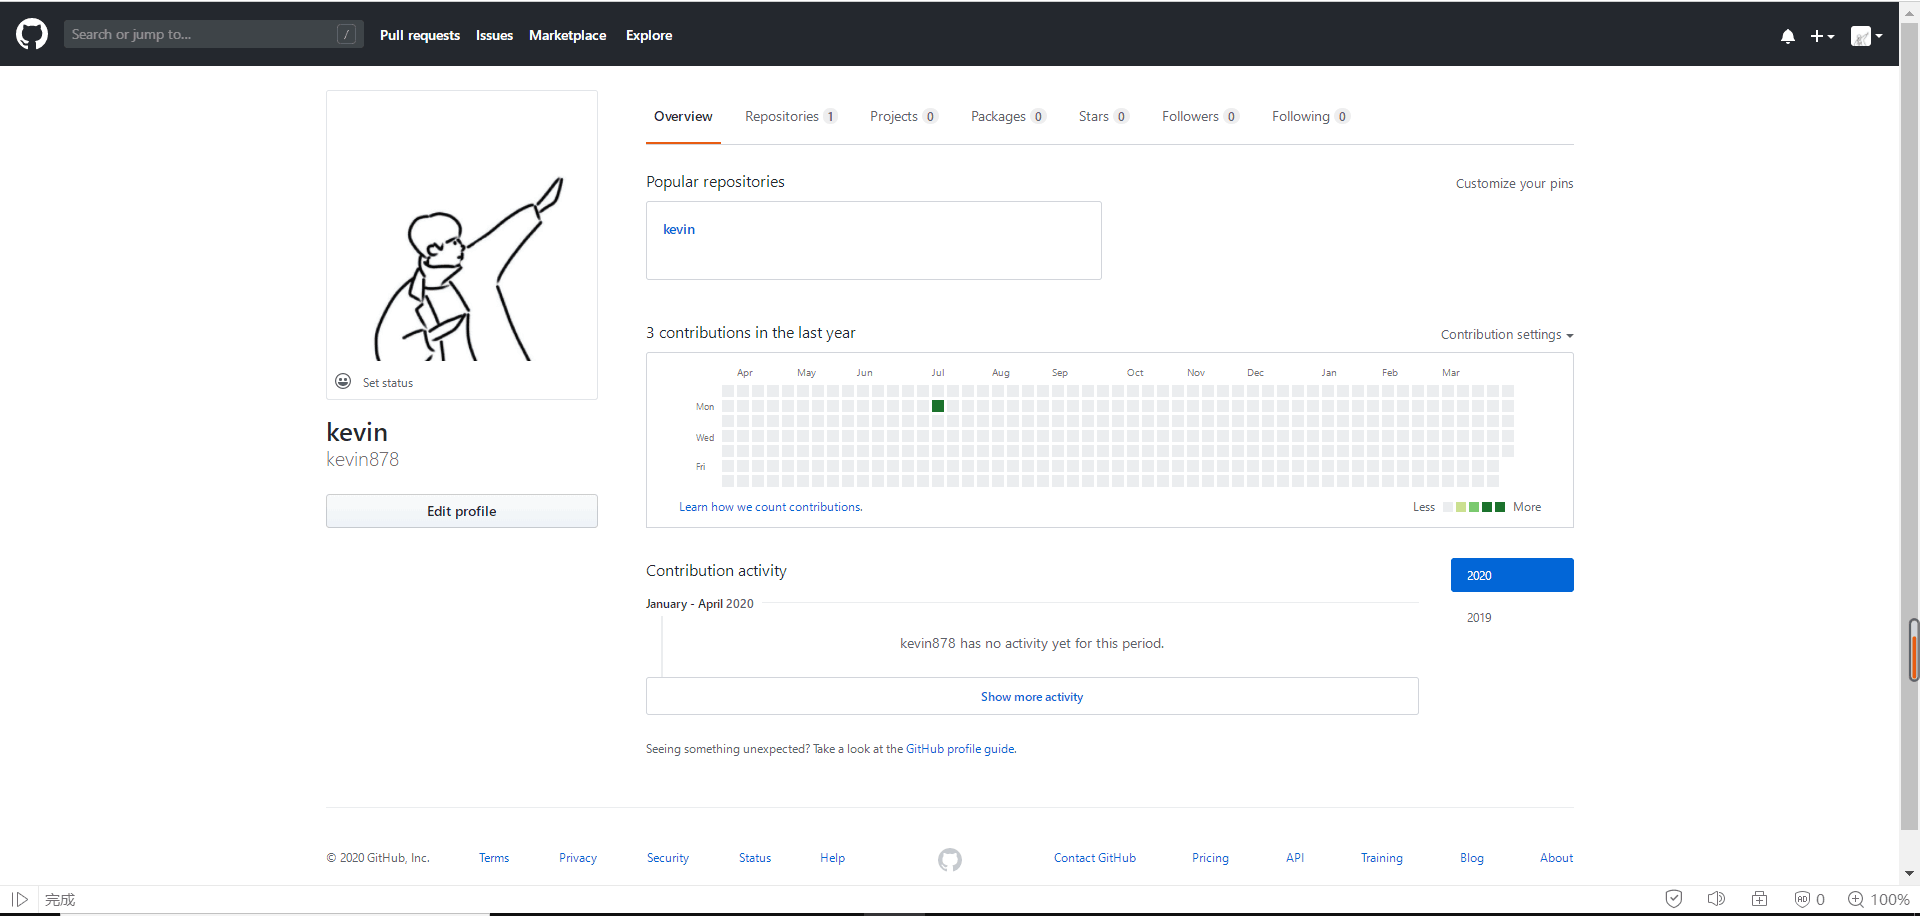
\includegraphics[scale=1.7]{github_account}
%\caption{The Universe}
%\label{fig:github_account}
%\end{figure}
	%插入图象
	%	\includegraphics{360wallpaper}
	%	
	%	\includegraphics[scale=0.3]{360wallpaper}
	%	
	%	\includegraphics[height=2cm]{360wallpaper}
	%	
	%	\includegraphics[width=2cm]{360wallpaper}
\begin{center}
	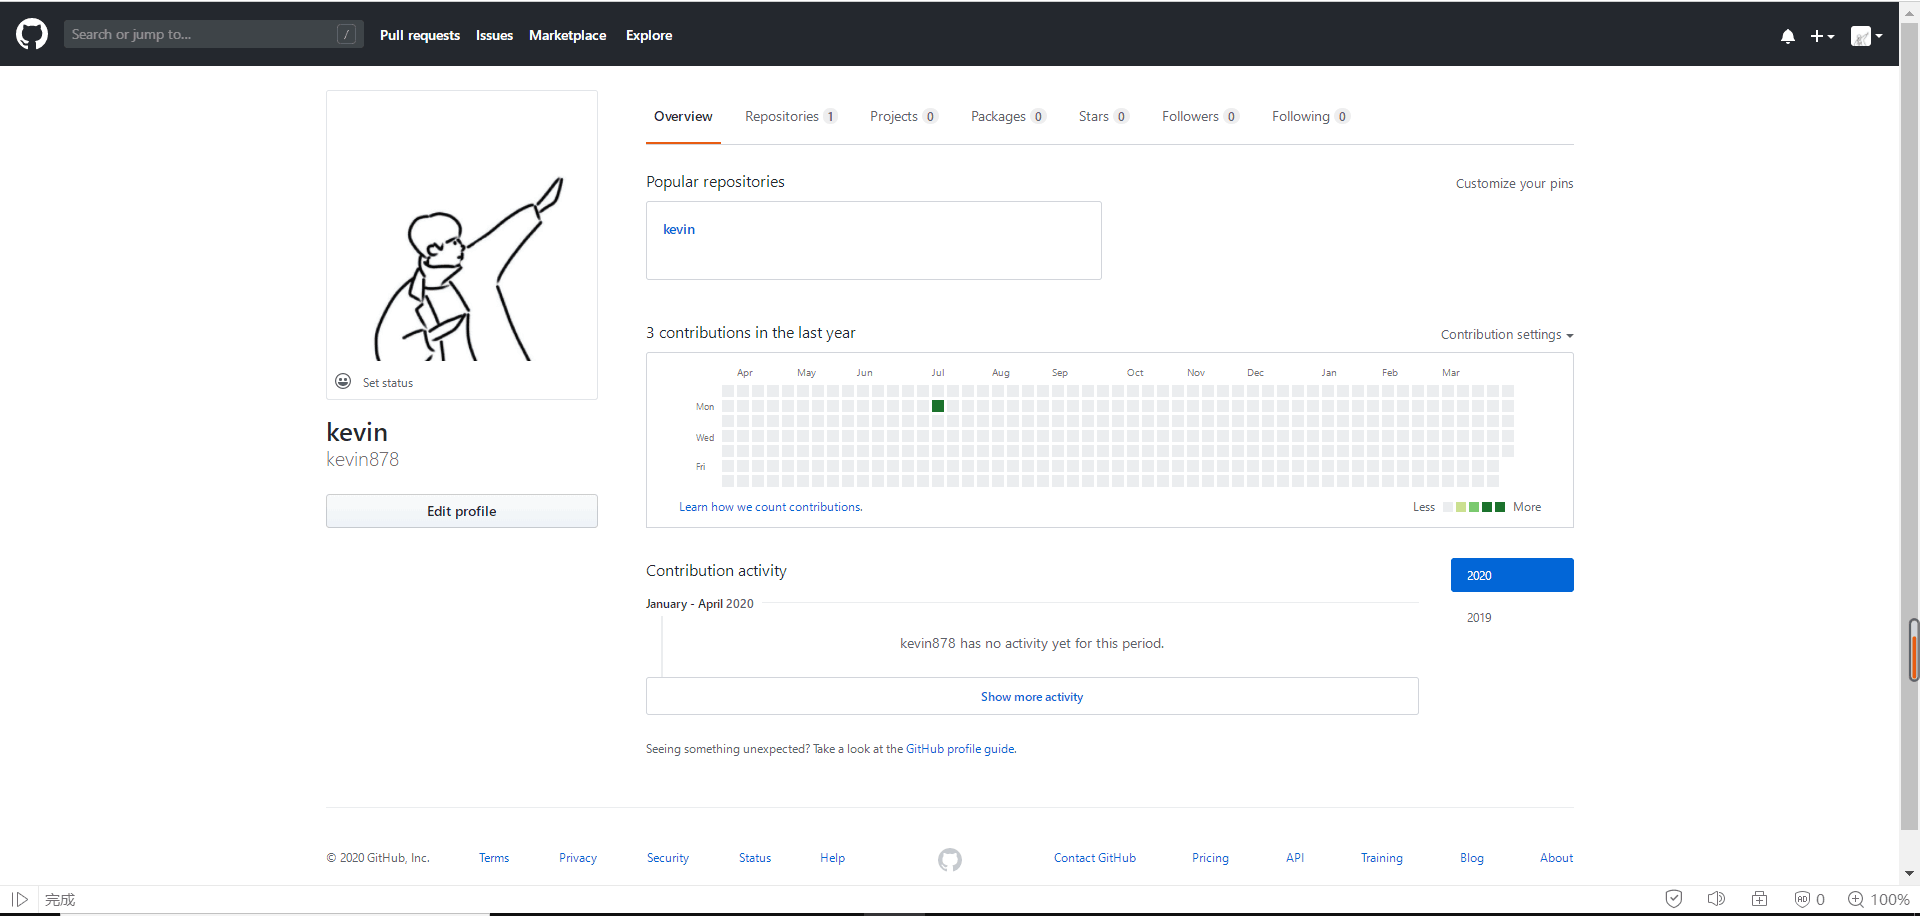
\includegraphics[scale=0.2]{github_account}
\end{center}
\subsection{学习强国截图}
\begin{center}
	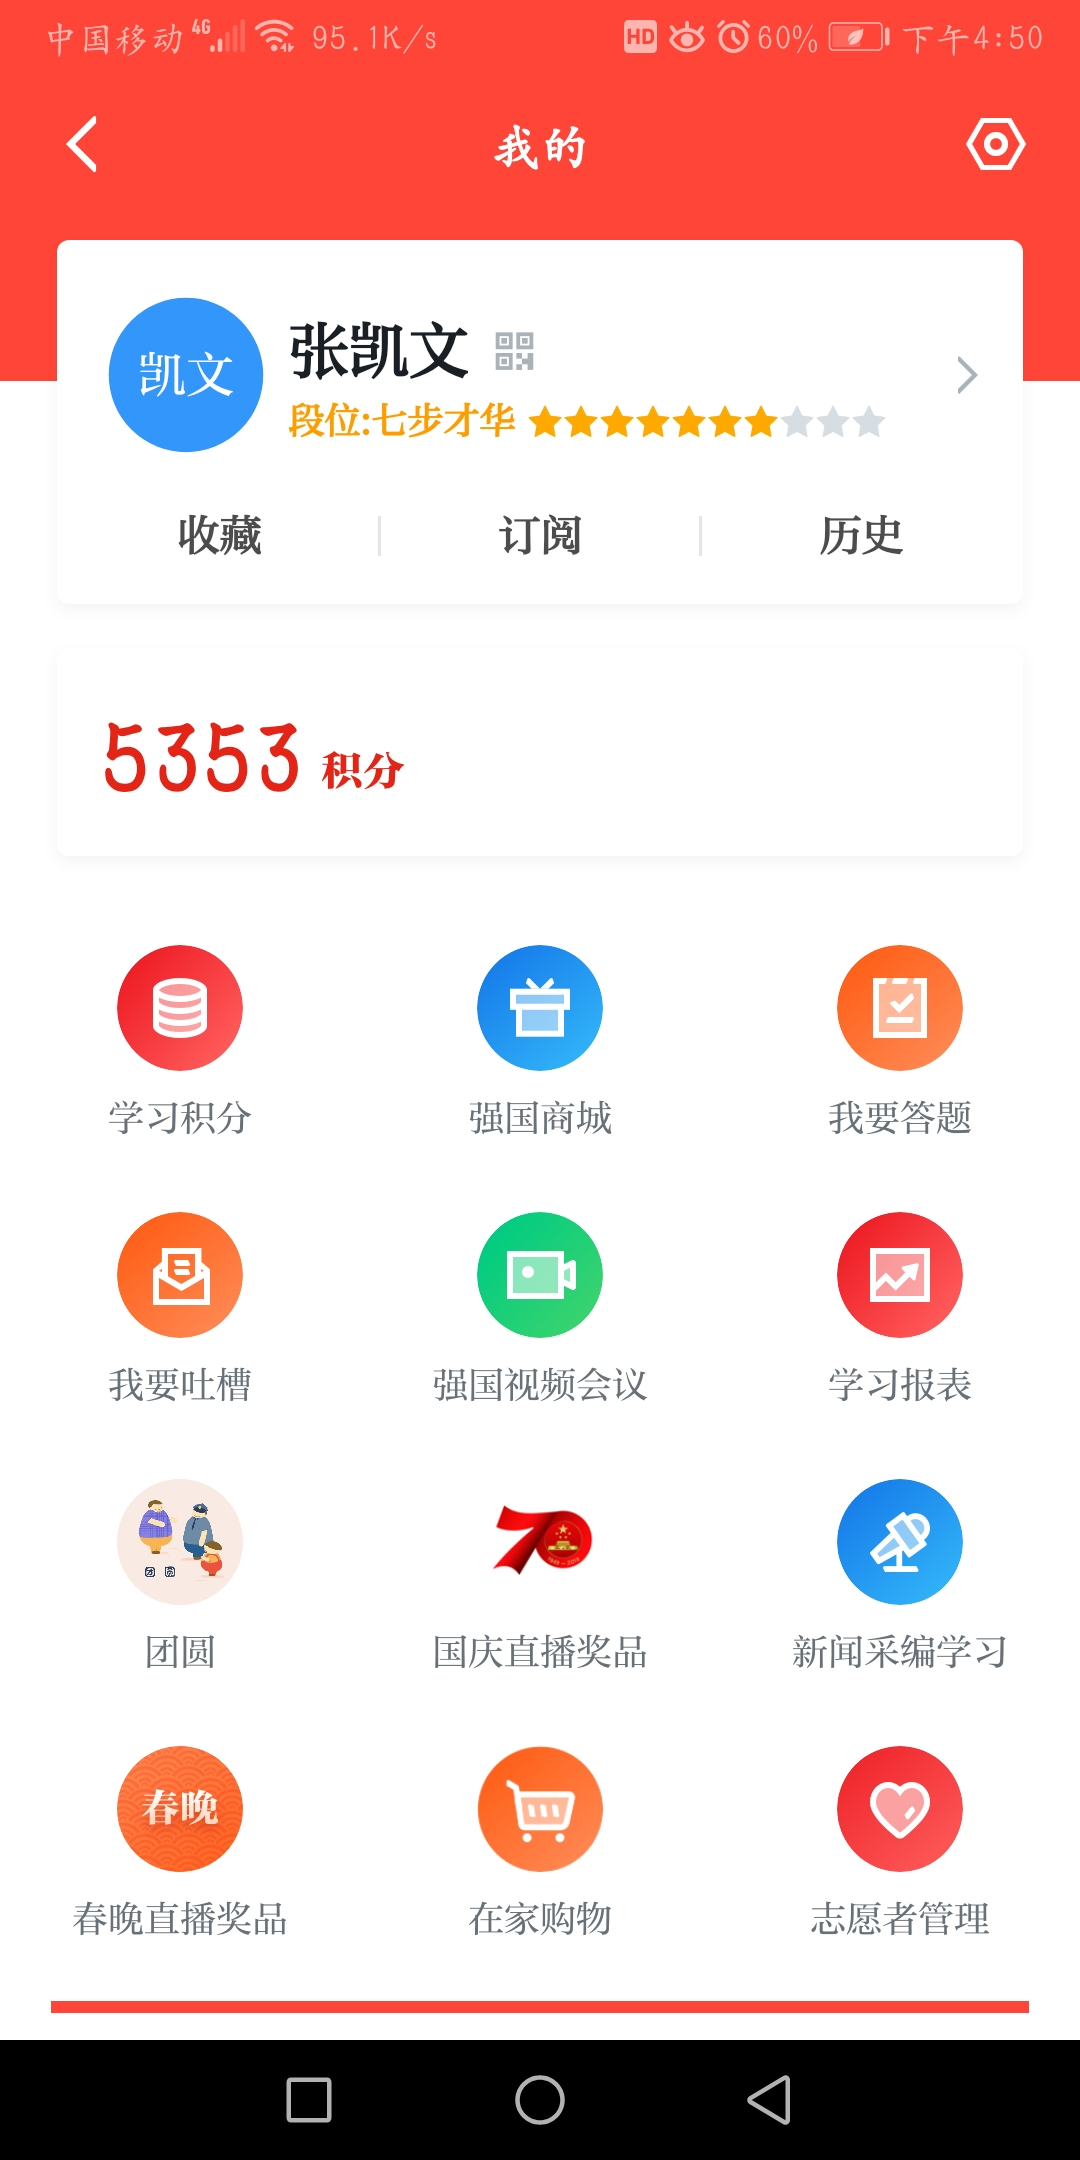
\includegraphics[scale=0.1]{xuexiqiangguo}
\end{center}

\hspace*{\fill} \\

%{\bf 注意,参考文献至少五篇,其中至少两篇为英文文献,参考文献必须在正文中有引用。}
\bibliographystyle{plain}
\bibliography{references}



\end{document}
